% !TEX root = ./Vortrag.tex
\begin{frame}[label=title]{}
\titlepage
%\begin{center} Betreuer: Benjamin Reh \& Thomas Kloepfer
%\end{center}
\end{frame}
\begin{frame}[label=title]{}
\tableofcontents
\end{frame}

\section{Projektziel}
\begin{frame}{Projektziel}
\begin{exampleblock}{Zielvorgaben}
\begin{itemize}
\item Konstruktion eines POV Globus
\begin{itemize}
\item Stabile Anzeige ohne Walk-Off
\item Einfaches Einlesen/Anzeigen von Bildern
\end{itemize}
\end{itemize}
\end{exampleblock}
\vspace{0.5cm}
\begin{exampleblock}{Umsetzung}
\begin{itemize}
\item Steuerung durch einen Raspberry Pi
\item Adafruit Dotstar LED Strip
\item Standventilatormotor als Antrieb
\item Programmierung in Python
\end{itemize}
\end{exampleblock}
\end{frame}

\section{POV-Prinzip}
\begin{frame}{Persitence Of Vision (POV)}
\begin{exampleblock}{}
\begin{itemize}
\item Das Auge kann Reize nur mit einer bestimmten Frequenz verarbeiten
\begin{itemize}
\item[]\Rightarrow Eine schnell bewegte Lichtquelle wird als Linie wahrgenommen
\item[]\Rightarrow Eine schnell bewegte, \emph{blinkende} Lichtquelle wird als mehrere Pixel wahrgenommen
\end{itemize}
\item Schnell rotierender Kreis \Rightarrow Kugeloberfläche
\item + (synchron zur Drehfrequenz) blinkende LED-Zeile \Rightarrow POV-Globe 
\end{itemize}
\end{exampleblock}
\end{frame}

\section{Komponenten}
\begin{frame}{Komponenten}
\vspace*{-1.35cm}
\begin{figure}
\hspace*{3cm}
%\center
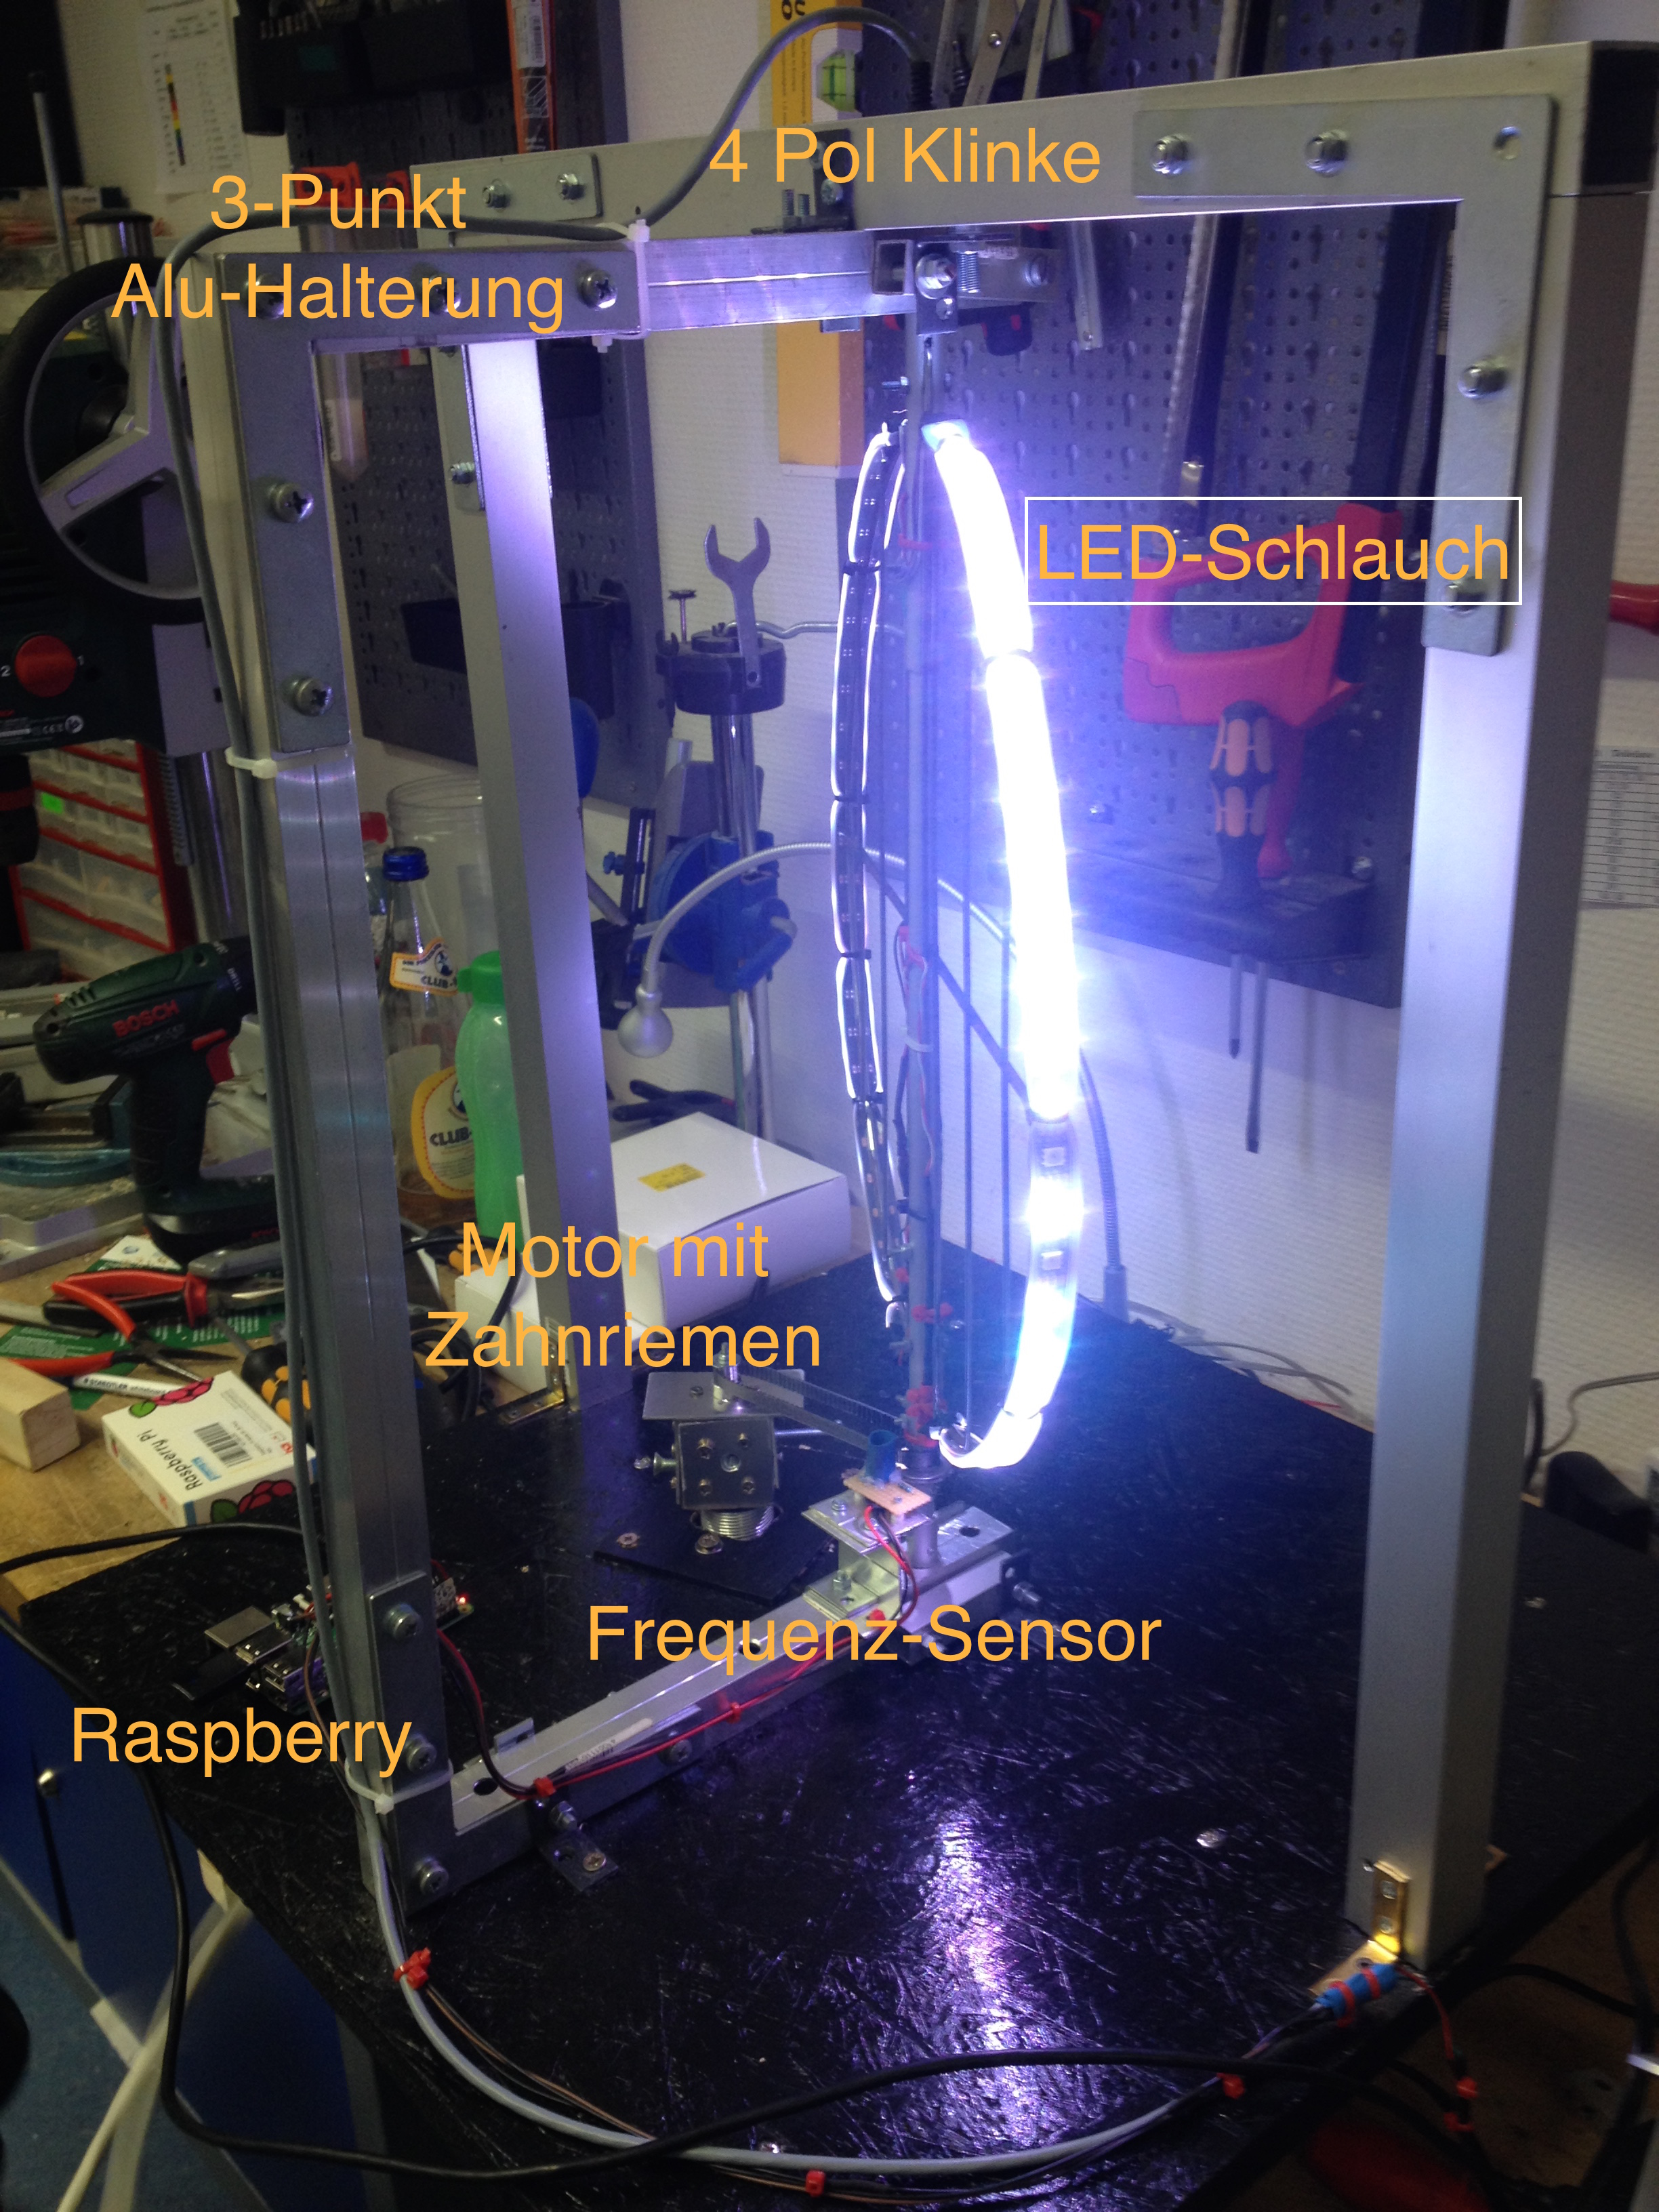
\includegraphics[height=1.19\textheight]{Plots/Komponenten.jpg}
\end{figure}
\end{frame}

\begin{frame}{}
\vspace*{-.5cm}
\begin{figure}
\center
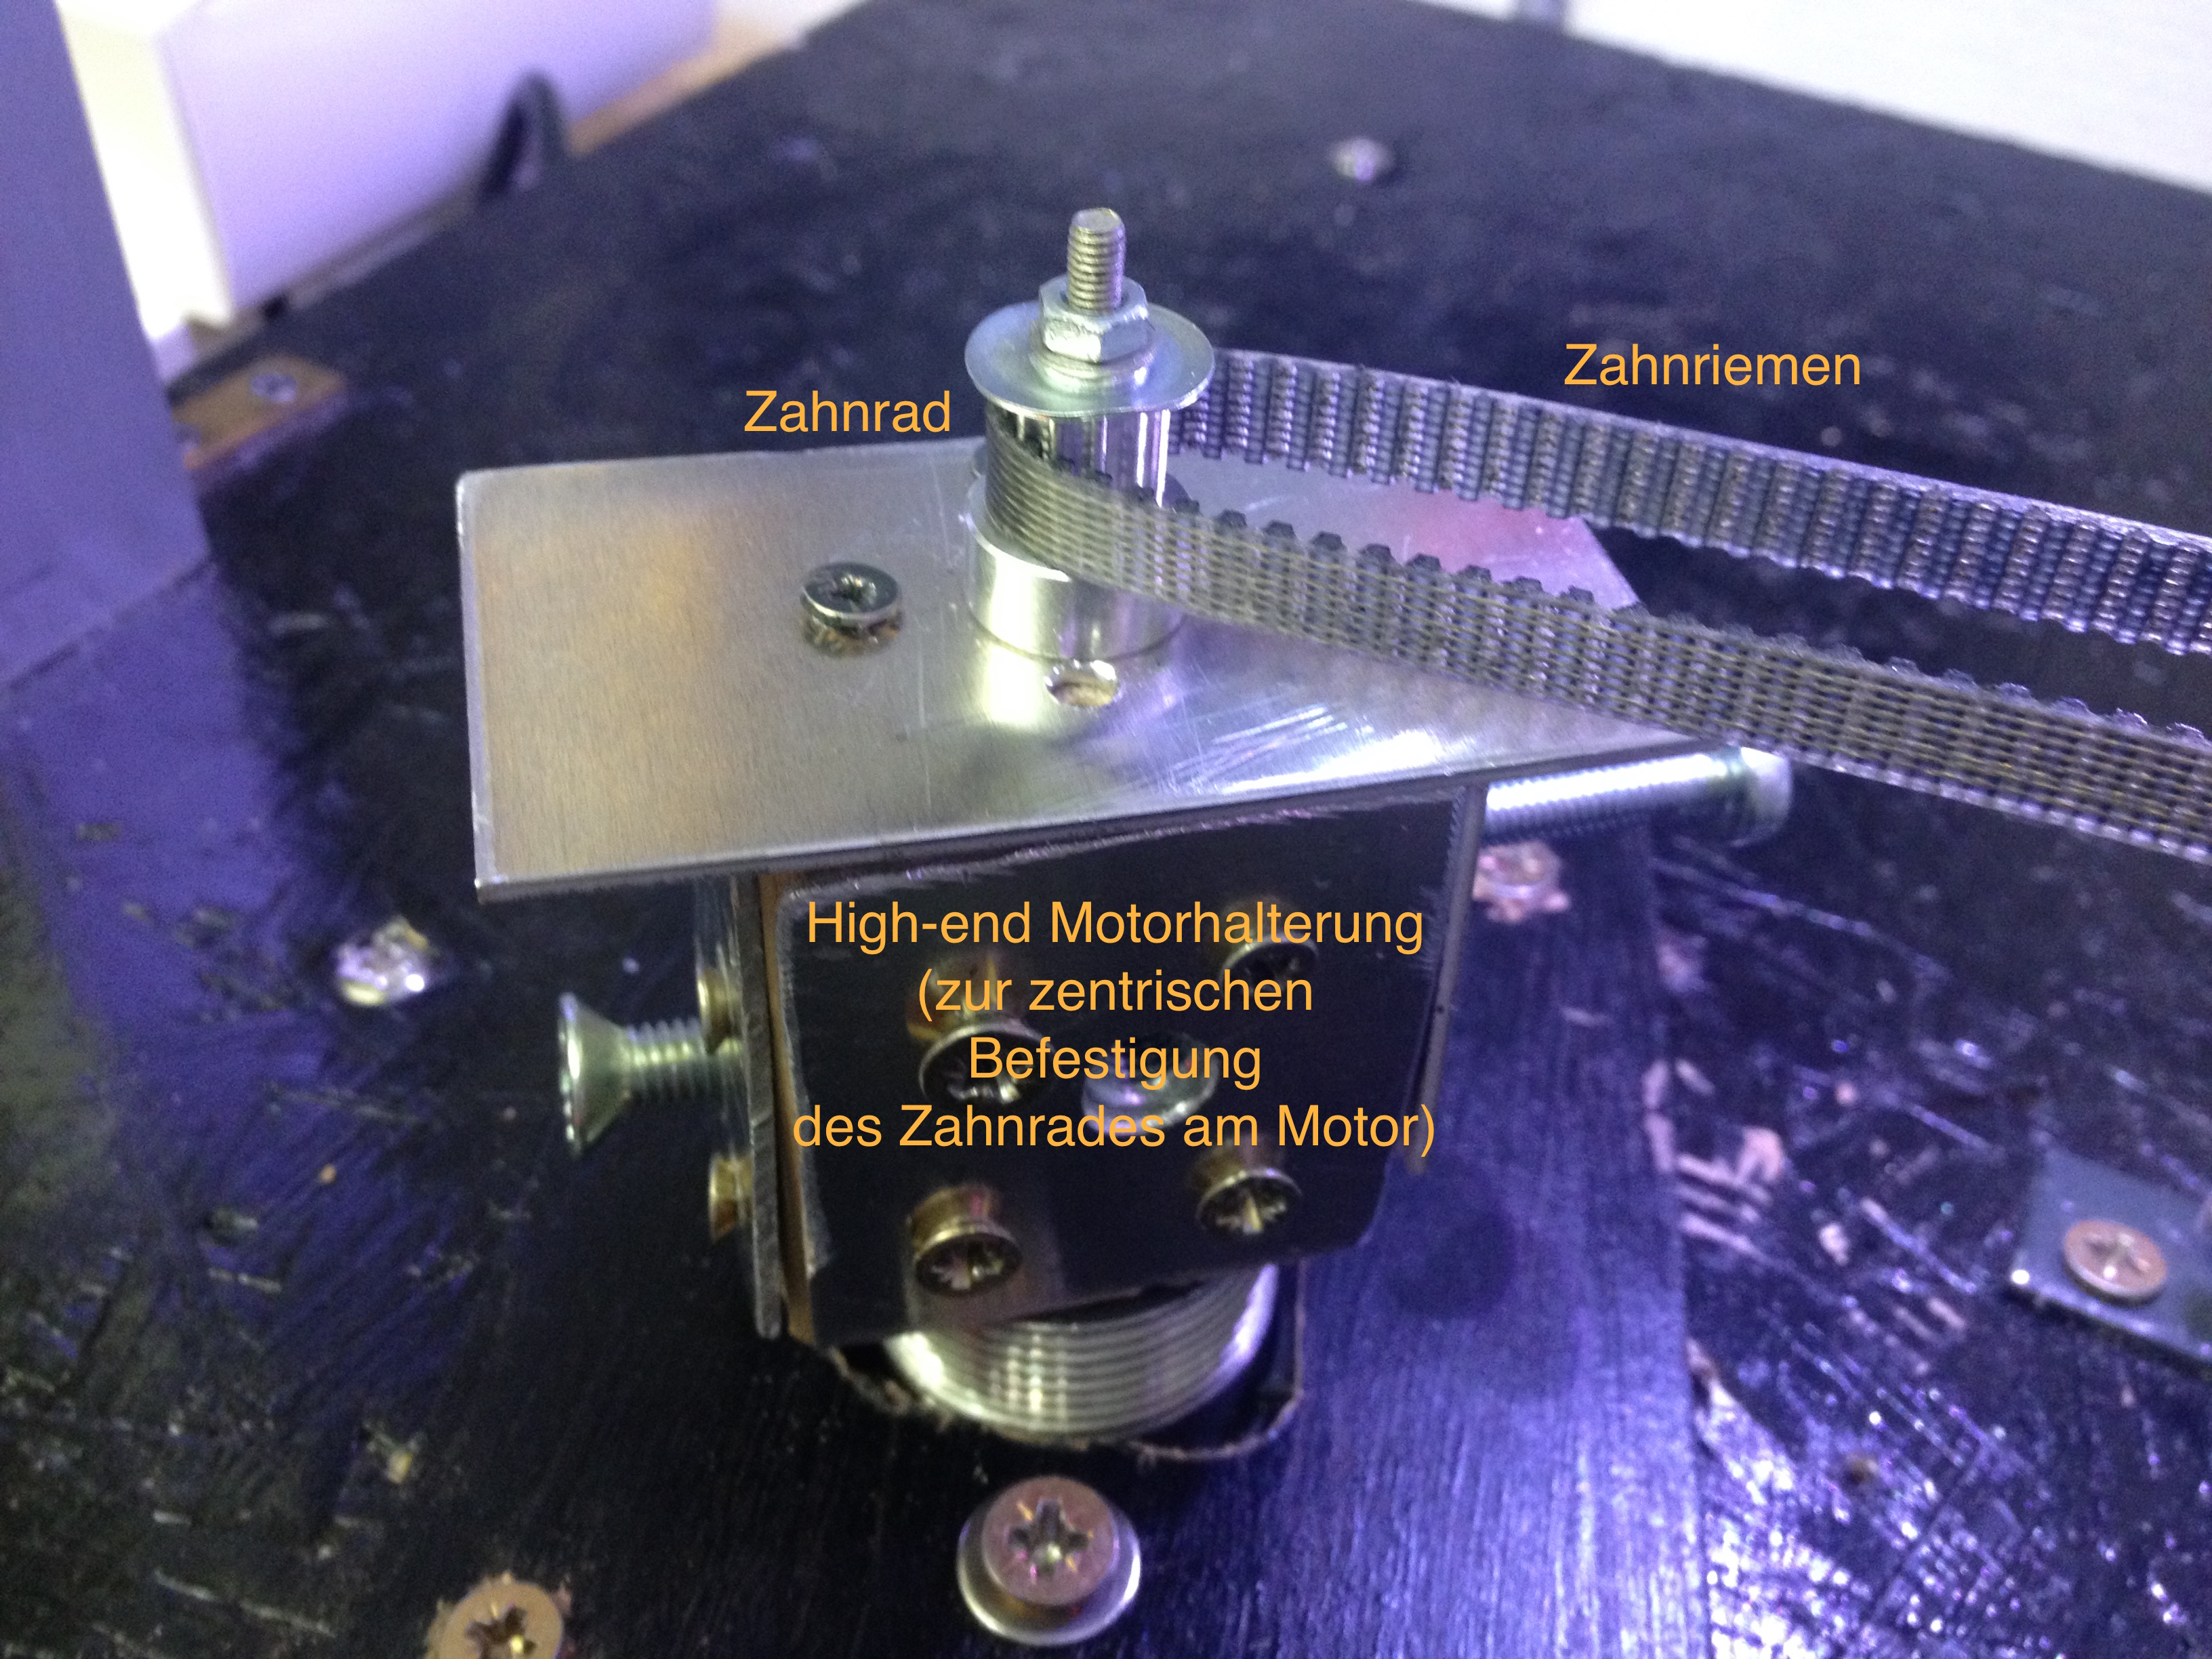
\includegraphics[height=\textheight]{Plots/Motor_oben}
\end{figure}
\end{frame}

\begin{frame}{}
\vspace*{-.5cm}
\begin{figure}
\center
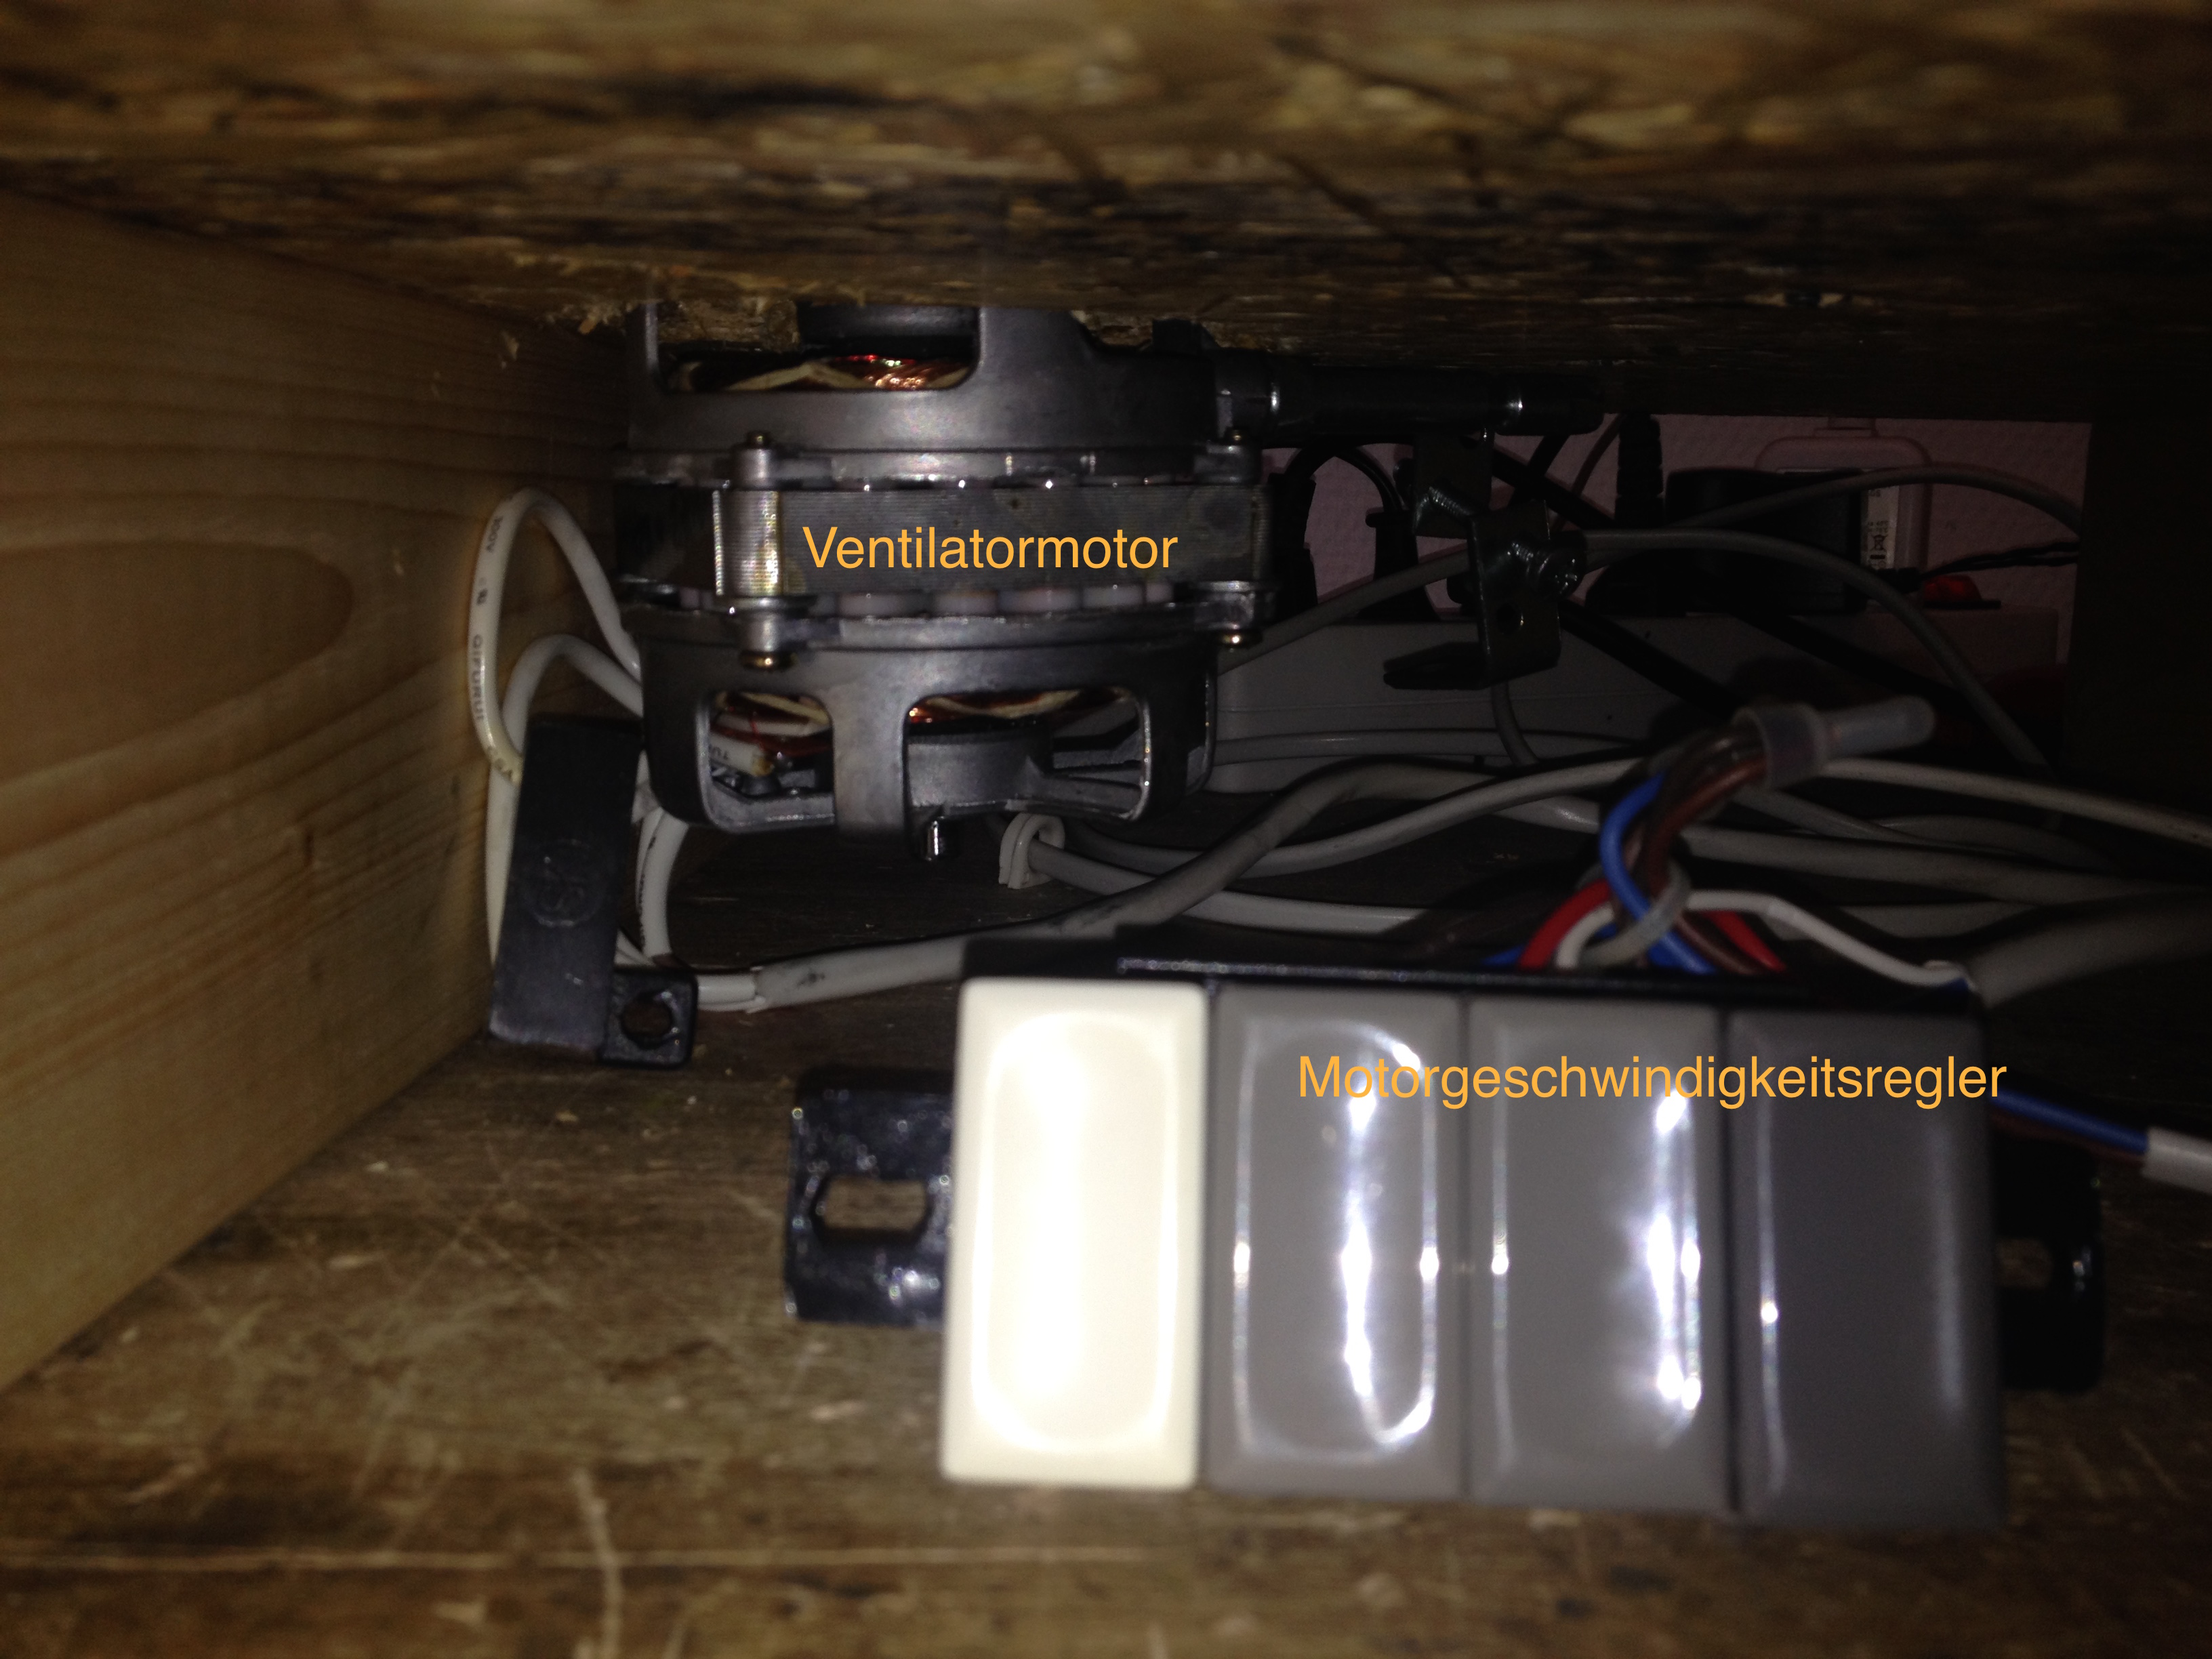
\includegraphics[height=\textheight]{Plots/Motor}
\end{figure}
\end{frame}

\begin{frame}{}
\vspace*{-.5cm}
\begin{figure}
\hspace*{-.5cm}
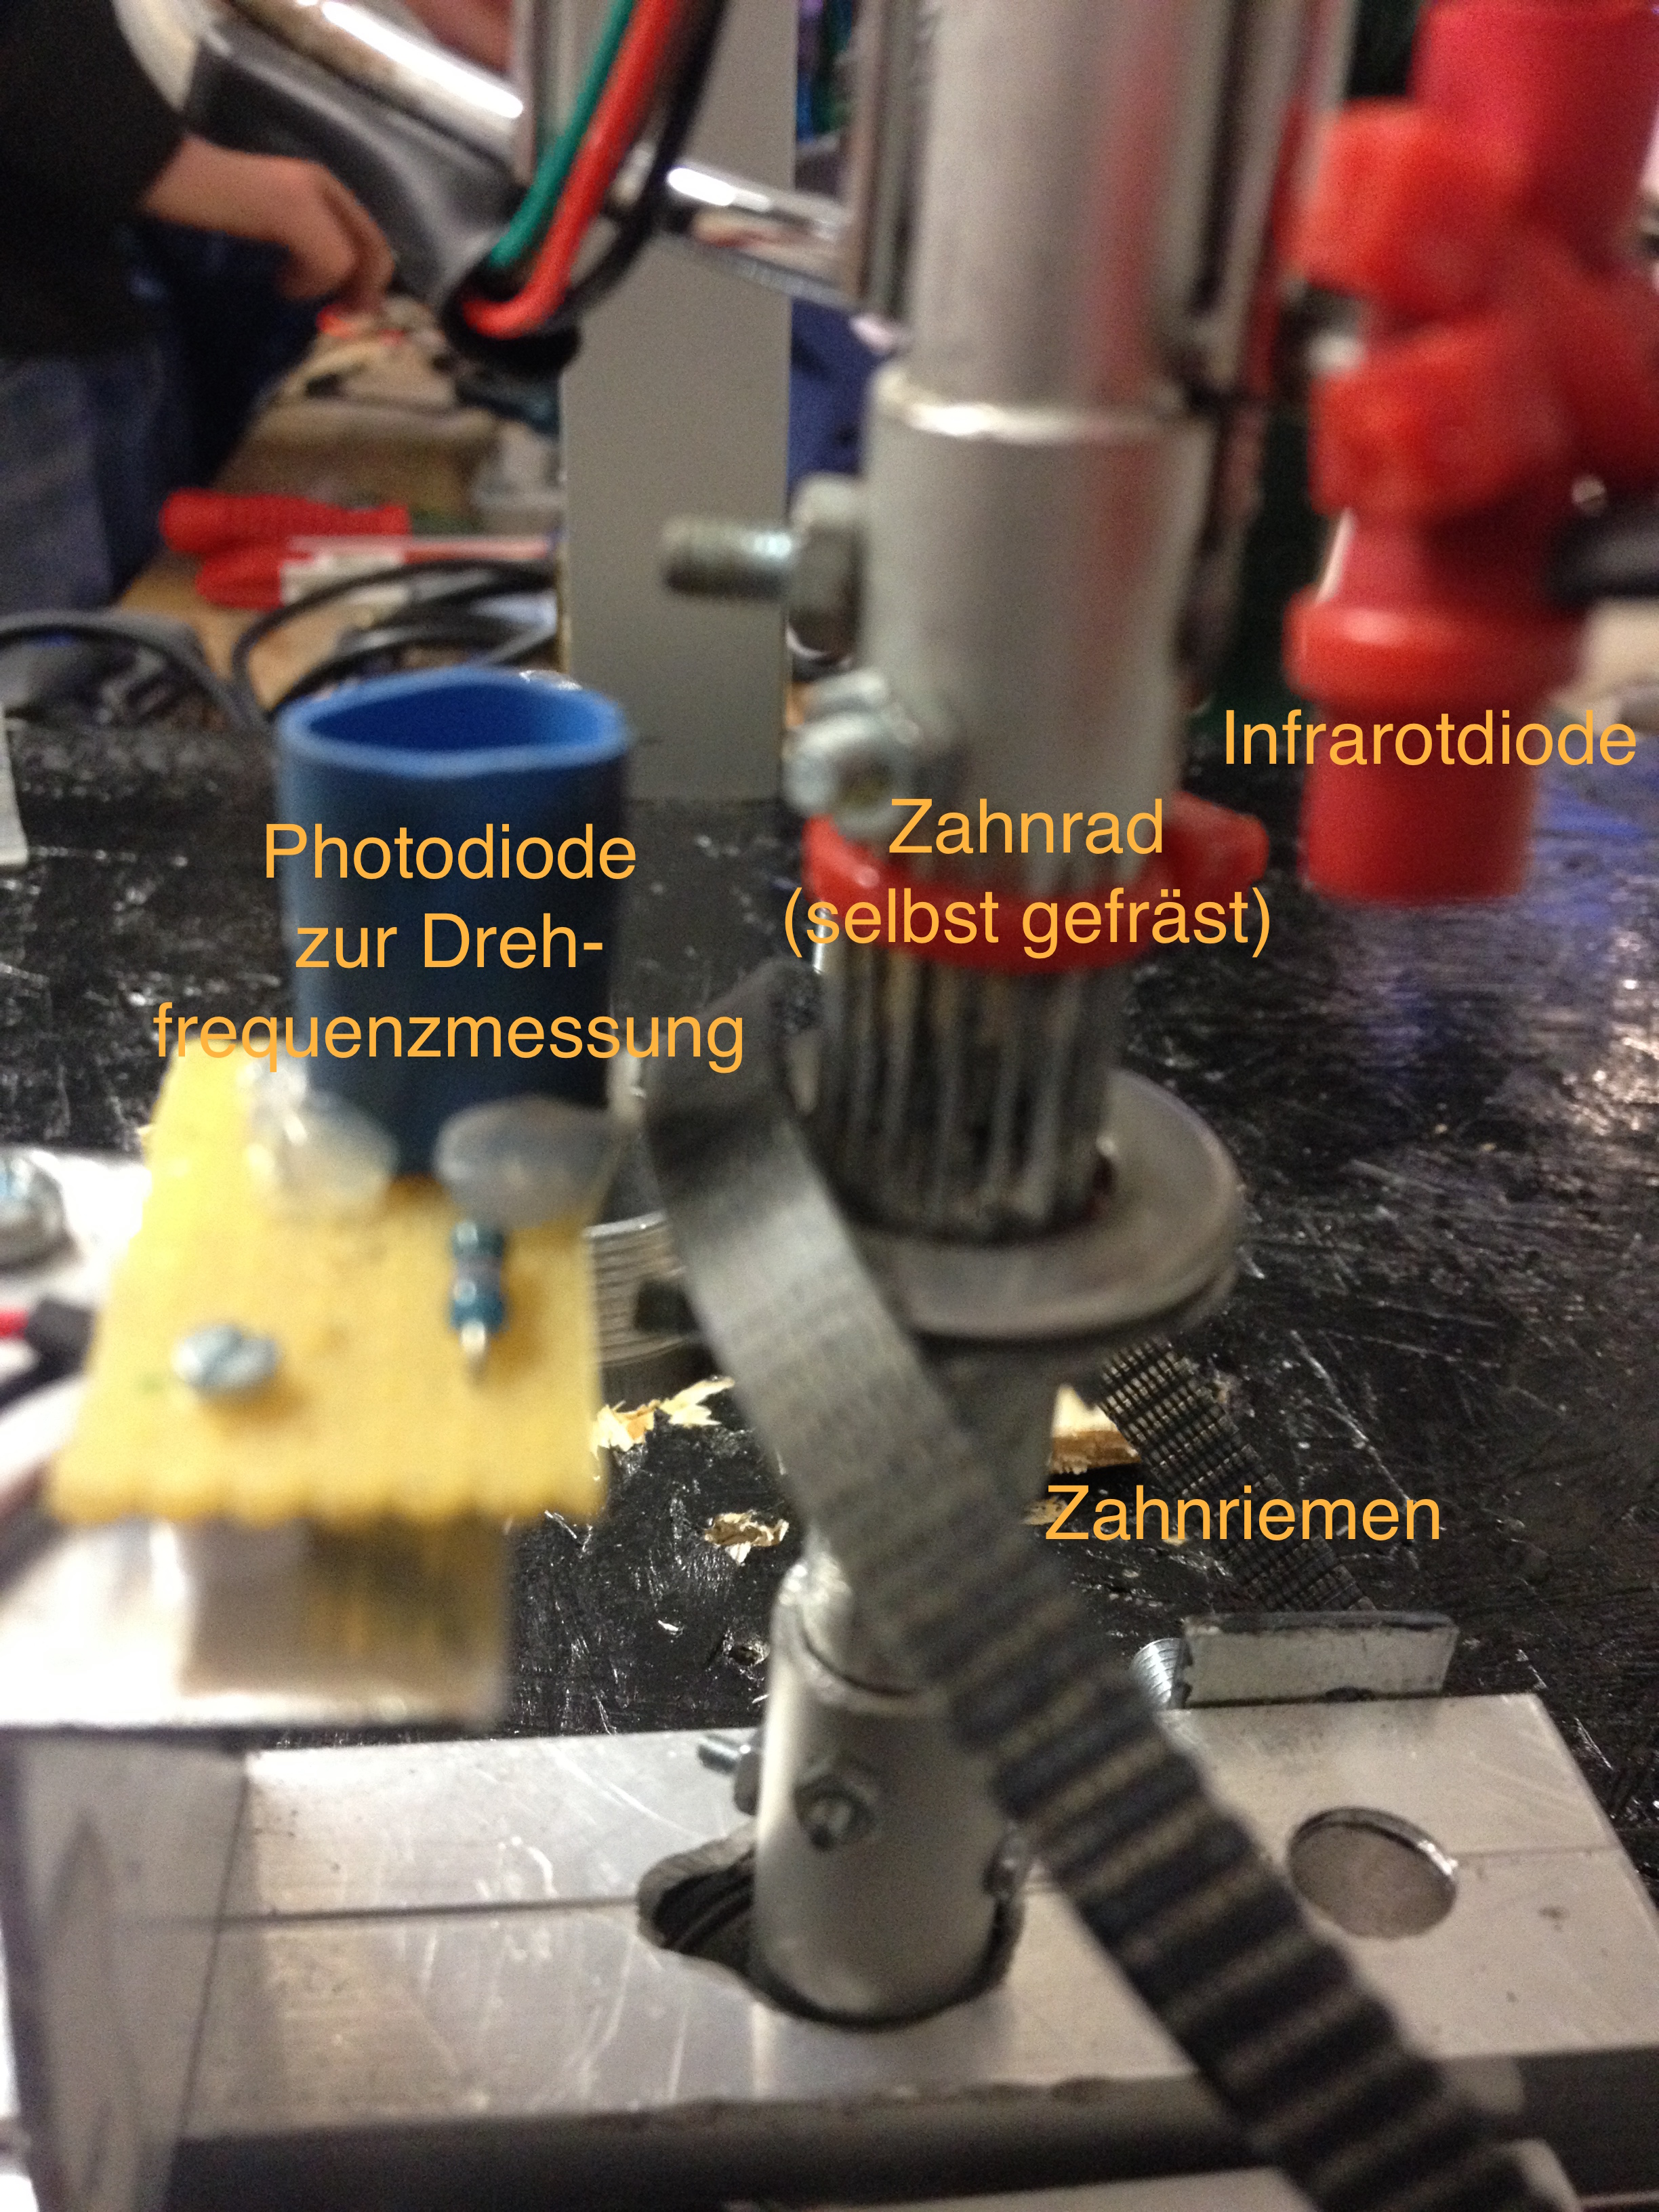
\includegraphics[width=.525\textwidth]{Plots/Zahnriemen}
\hspace*{.1cm}
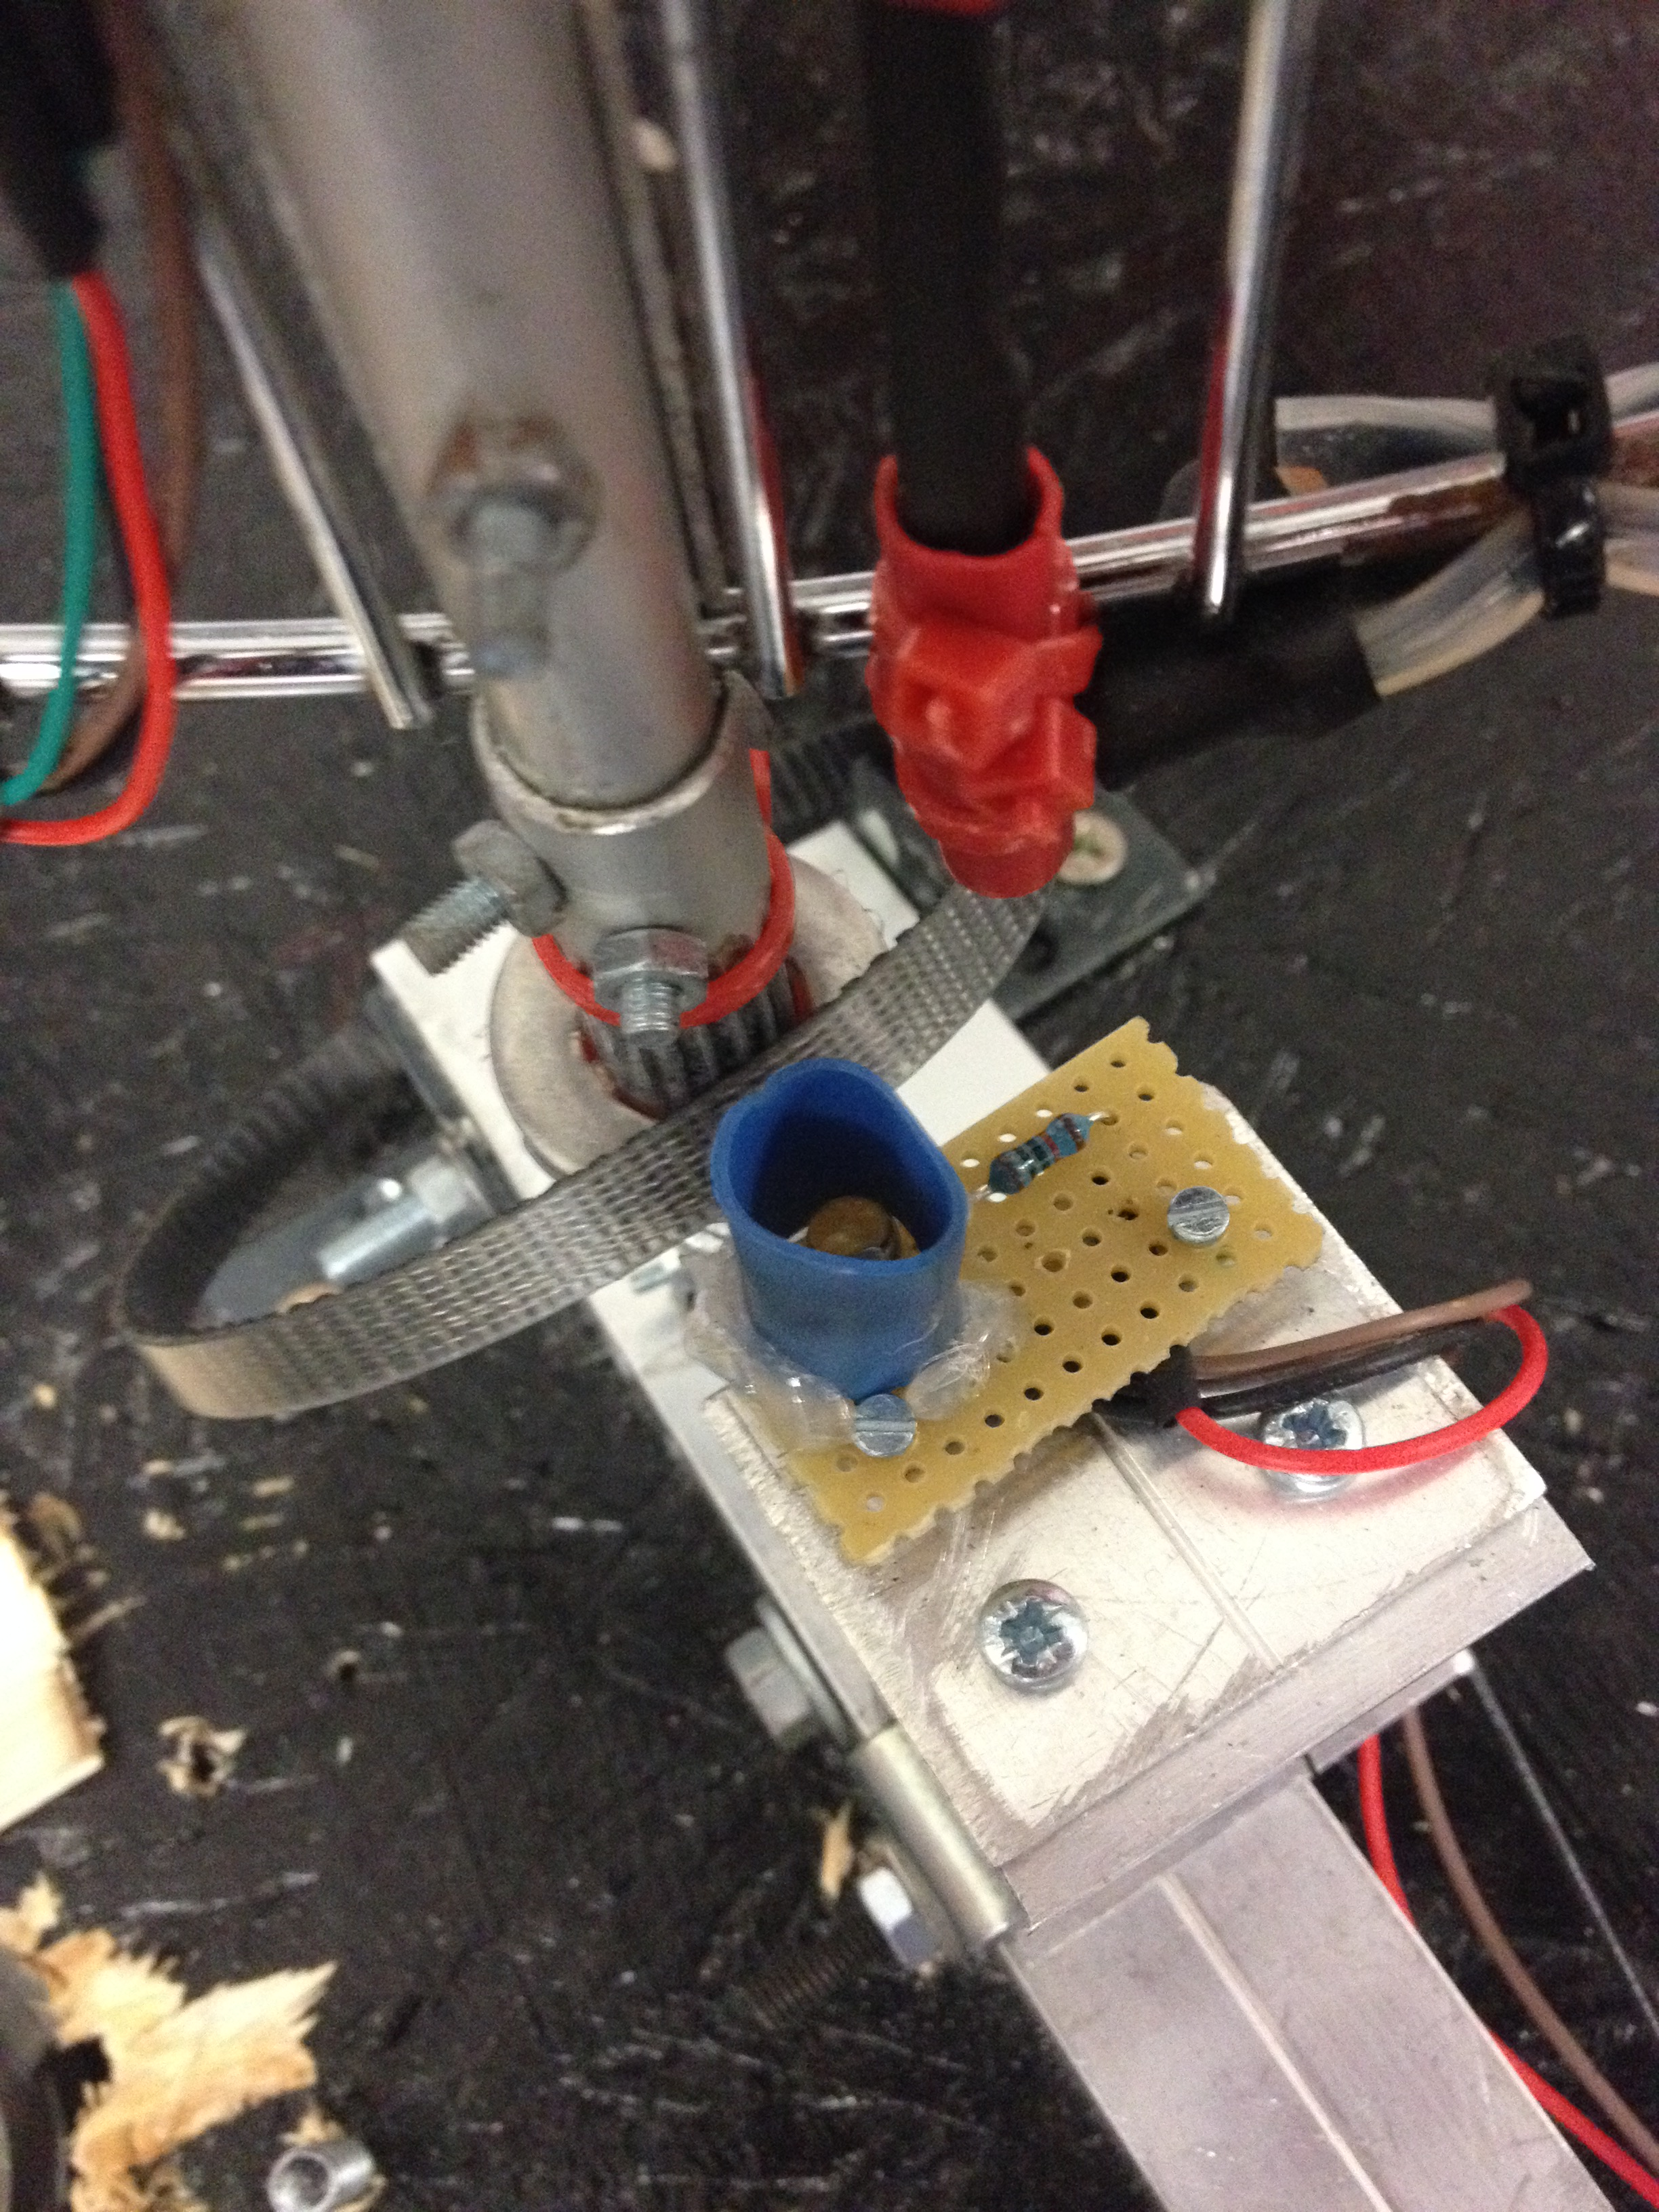
\includegraphics[width=.525\textwidth]{Plots/Photodiode}
\end{figure}
\end{frame}

\begin{frame}{}
\vspace*{-.5cm}
\begin{figure}
\center
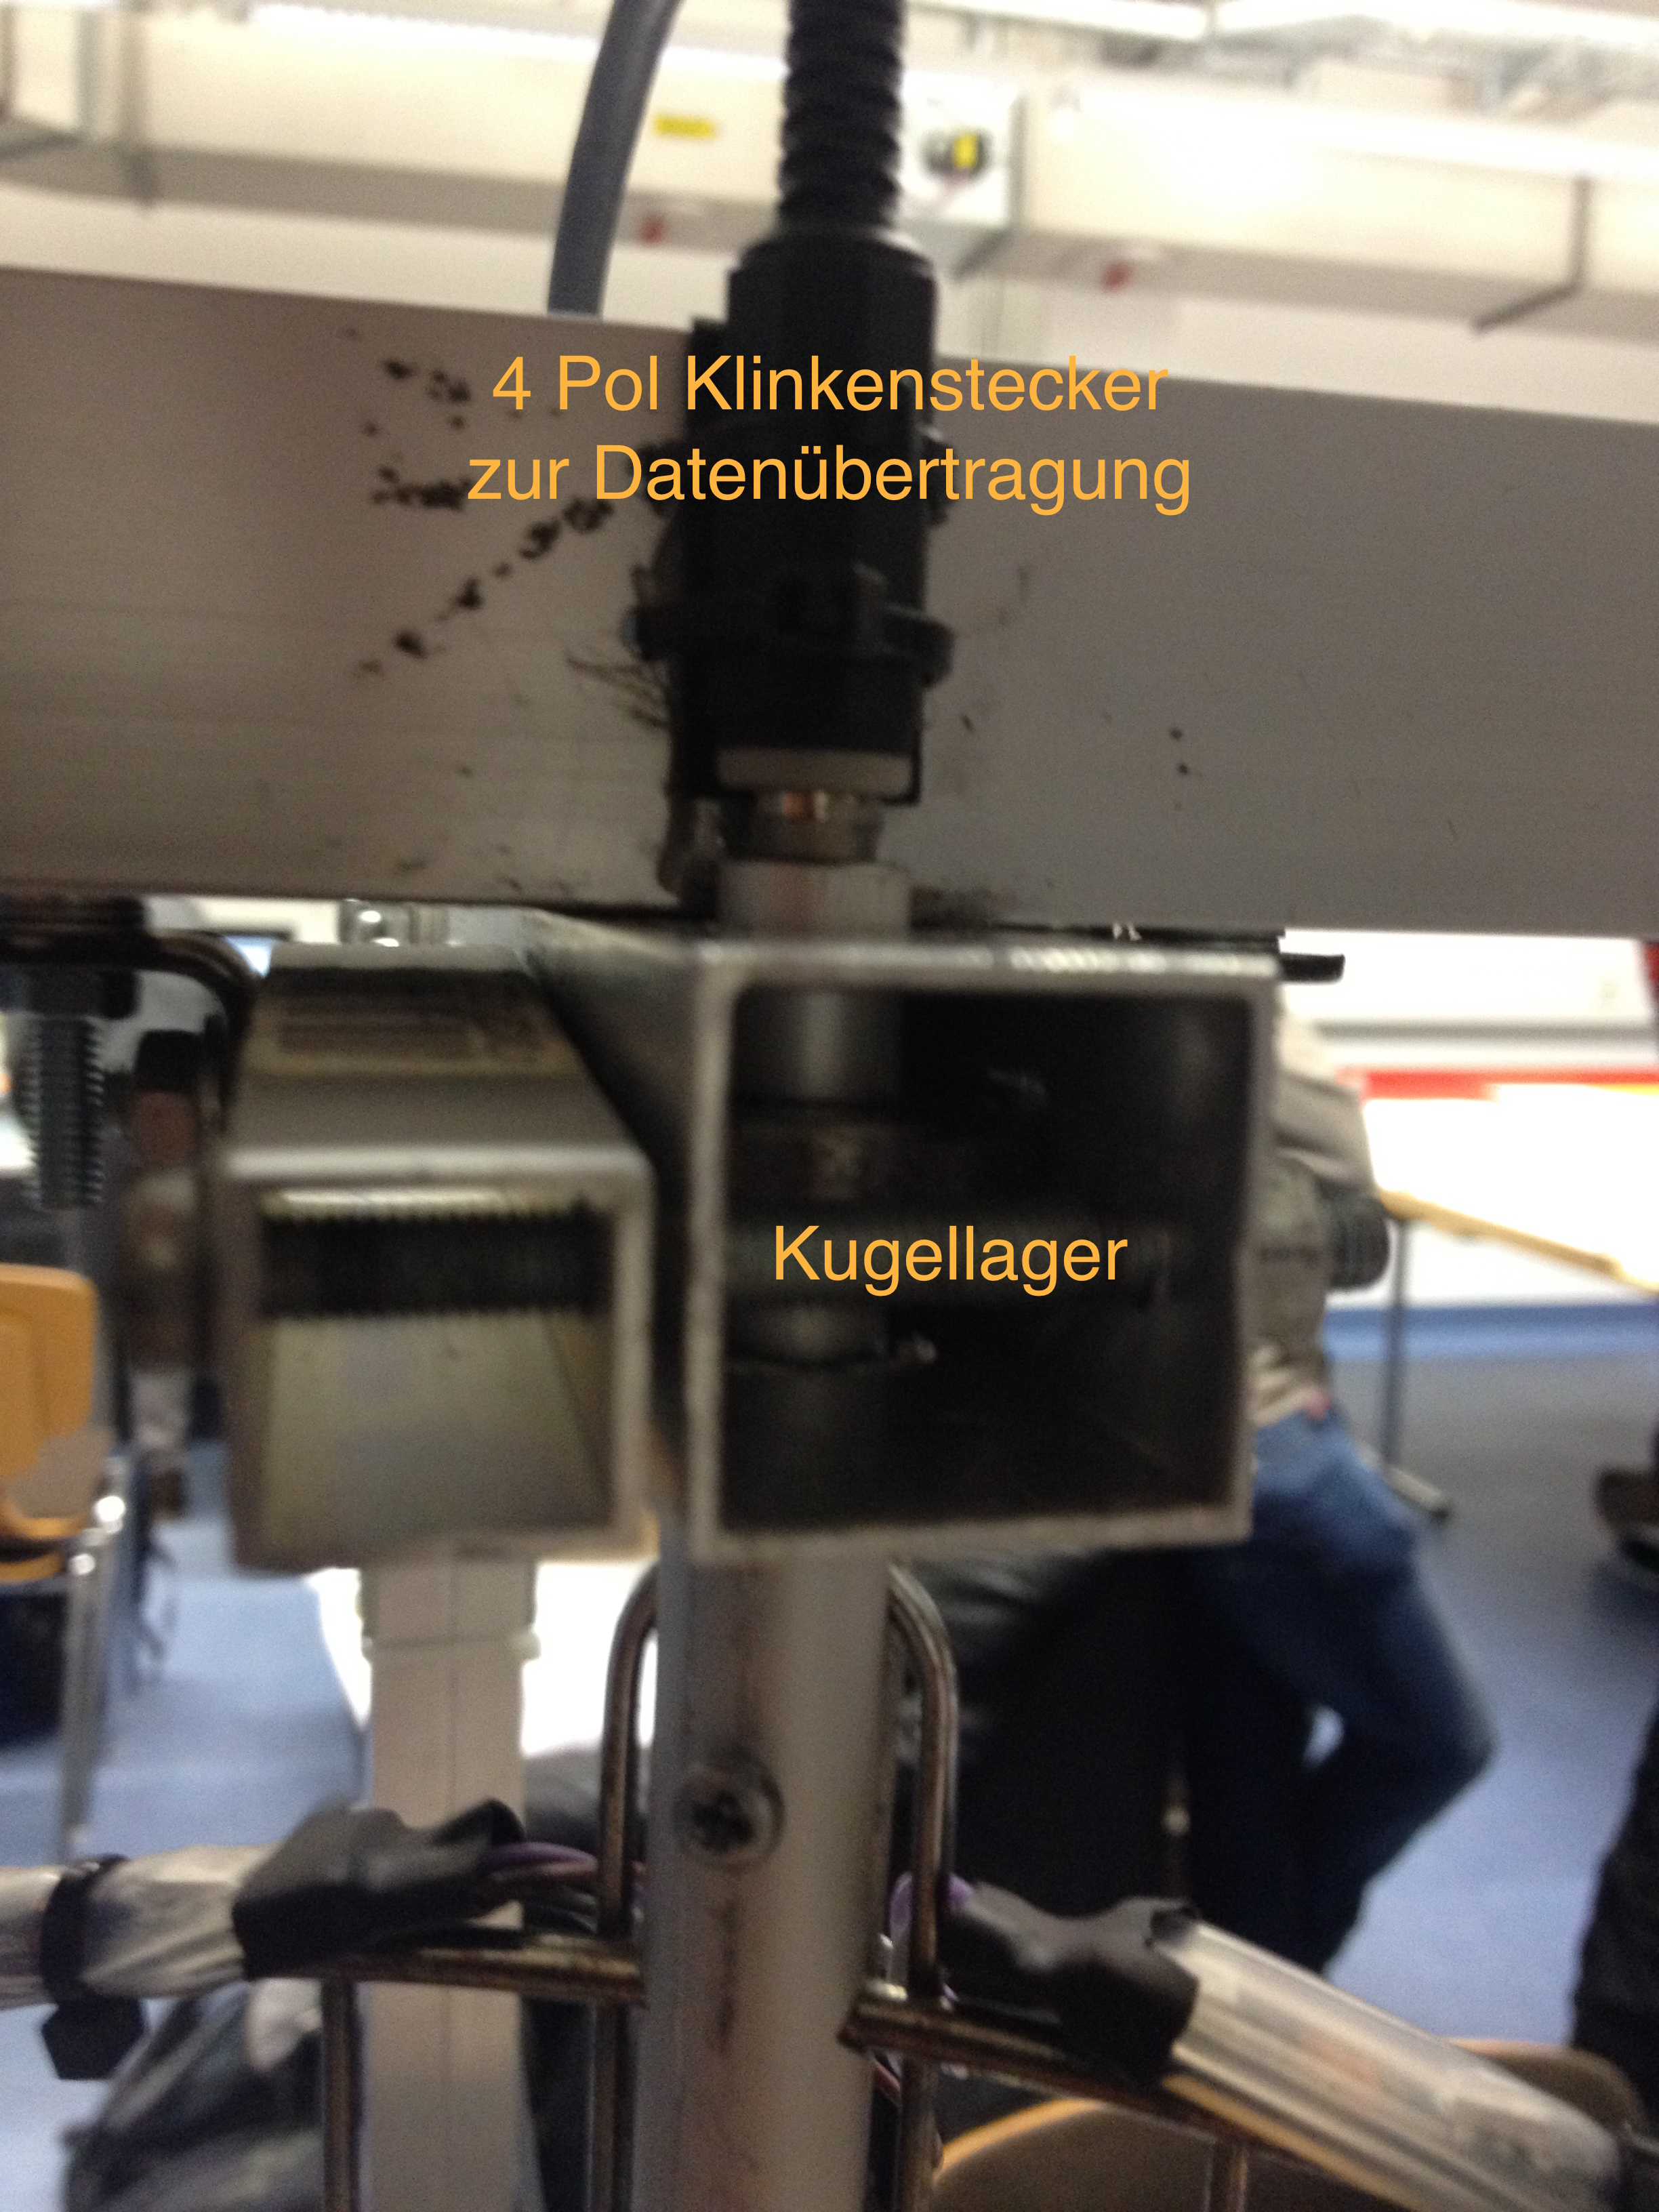
\includegraphics[height=\textheight]{Plots/Klinke}
\end{figure}
\end{frame}

\begin{frame}{Features}
\begin{exampleblock}{}
Datenübertragung über 4 Pol Klinke (axial gelagert)
\begin{itemize}
\item Idee: Nur der LED-Schlauch soll rotieren
\item LED Schlauch benötigt 4 Anschlüsse: VCC, GND, DATA, CLOCK 
\item Übertragung der Daten auf rotierende Elemente via 4 Pol Klinke
\end{itemize}
\end{exampleblock}
\end{frame}


\begin{frame}{POV}
%\begin{listings}
%\end{listings}
\lstinputlisting[firstline=10,lastline=20]{show_pov.py}
\end{frame}

\begin{frame}{Sensor-Thread}
\begin{itemize}
\item Abfragereihenfolge: links, oben, rechts, oben, links, ...
\item Bei Abfrage oben, drehe den Servo weiter nach rechts
\item Am rechten Rand, springe nach links \\[0.5cm]
\item Speichere aktuelle Sensordaten in Array
\item Ignoriere Werte kleiner als 7cm
\item Fünf Versuche für korrekte Messung
\end{itemize}
\end{frame}

\section{Probleme}

\begin{frame}{Probleme}
\begin{itemize}
\item Probleme mit diversen Motoren
\item[] \rightarrow diverse Konzepte ausprobiert
\item Datenübertragung
\item Lagerung des Kreises
\item zentrische Lagerung der gesamten Konstruktion
\end{itemize}
\end{frame}

\section{Ausblick}

\begin{frame}{Ausblick}
\begin{itemize}
\item Verbesserung der Bildverarbeitung
\begin{itemize}
\item bewegte Bilder
\item Schrift Übertragen
\item Spiele programmieren
\end{itemize}
\item bessere Lagerung
\item besserer Motor
\item höhere Anzahl an Pixel
\end{itemize}
\end{frame}

\begin{frame}
\begin{center}
\textcolor{darkred}{
Vielen Dank für Ihre Aufmerksamkeit}
\end{center}
\end{frame}
